\documentclass{article}
\author{Alex Hiller}
\title{Foundation Mathematics U:PASS}
% Type-setting
\setlength{\parindent}{0cm}
\setlength{\parskip}{0.125cm}
\pagenumbering{gobble}
\usepackage[margin=2.5cm]{geometry} % Formatting

% Packages
\usepackage{amsmath}                  % Mathematics
\usepackage{amssymb}                  % Mathematics
\usepackage{listings}                 % Listings
\usepackage{esint}
\usepackage{color}                    % Listings
\usepackage{courier}                  % Listings
\usepackage{circuitikz}               % Circuits
\usepackage{titlesec}                 % Section Formatting
\usepackage{graphicx}

% Code Formatting 
\input{/home/polluticorn/GitHub/texTemplates/codeFormat}
% Math Macros
\input{/home/polluticorn/GitHub/texTemplates/mathMacros}
% Note Taking Macros
\input{/home/polluticorn/GitHub/texTemplates/noteTaking}

% Section formatting
\titleformat{\section}{\large \bfseries}{}{0em}{}[]
\titleformat{\subsection}{\Large \bfseries}{}{0em}{}
\titleformat{\subsubsection}{\bfseries}{}{0em}{}


\begin{document}

\maketitle

\section{Question 1}
Sketch (to the right) the inverse of the function below.
\begin{figure}[h!]

  \includegraphics[width=0.4\linewidth]{function.pdf}
\end{figure}

\section{Question 2}
Differentiate the following functions:
\begin{equation}
  \frac{x^{4}_{} }{4} + \frac{x^{3}_{} }{27}
\end{equation}

\begin{equation}
  \ln \big( x^{2} + 4 x + 5 \big)
\end{equation}

\begin{equation}
  \frac{x^3 + 4x^2 + 7}{4x^3 + 7x + 29}
\end{equation}

\begin{equation}
  \big( x - 2 \big) \big( x^4 + 39x^2 + 405 \big)
\end{equation}

\section{Question 3} 
Find:
\begin{equation}
  \lim_{n \rightarrow \infty} \bigg( 1 + \frac{1}{n}  \bigg)^n
\end{equation}

\section{Question 4}

\textbf{Derive} the following formulae related to geometric progressions:

\begin{equation}
  \text{Finding the $n$th term in the geometric progression.}
\end{equation}

\begin{equation}
  \text{Finding the partial sum up to the $n$th term.}
\end{equation}

\end{document}
